\chapter{Experiments}
\label{chap:experiments}

Having established our experimental setup and the environments we use, we move on to the experiments themselves. 
Firstly, we establish the benchmark scores for spectrograms, filterbanks and MFCCs.
Thereafter, we evaluate the quality of a single feature map obtained through the VGG16 network on spectrograms, filterbanks and MFCCs as input, as well as examine the qualitative properties of the top feature maps.
Finally, we combine the top features obtained to form a hybrid feature map and evaluate the quality of these combined features.

\section{Benchmark Scores}

In order to compare the quality of our newly acquired features, we need a benchmark score to compare it against. 
As stated in previous chapters, we use the AP scores obtained from the generic spectrograms, filterbanks and MFCCs of the Buckeye Corpus. 
Running the evaluation algorithm described in Chapter~\ref{chap:evaluation} on these features resulted in the AP scores shown in Table~\ref{tbl:benchmarks} and the precision-recall curves shown in Figure~\ref{fig:pr-curve}.

\begin{table}[!ht]
    \mytable
    \caption{Benchmark AP scores for Spectrograms, filterbanks and MFCCs.}
    \begin{tabularx}{0.85\linewidth}{@{}Ll@{}}
        \toprule
        Feature         & AP        \\
        \midrule
        Spectrograms    & $0.02347$ \\
        Filterbanks     & $0.1890$  \\
        MFCCs           & $0.2843$  \\
        \bottomrule
    \end{tabularx}
    \label{tbl:benchmarks}
\end{table}

As expected, spectrograms result in a very low AP score of 0.02347 due to the high variability caused by different speakers, tones, channels and acoustic conditions. 
Filterbanks result in a significant improvement on spectrograms with an AP score of 0.189 due to the reduced impact of frequency ranges that fall outside normal speech. 
MFCCs, with an AP score of 0.2843, further improve on filterbanks by removing much of the spectral noise found within filterbanks as well as added improvement through the use of the delta and delta-delta features.

To gain some insight into how similarity between two of the same words are represented within each of these features, Figure~\ref{fig:cost_matrix} shows the distance matrix between two spoken phrases of the word ``graduate" calculated during Algorithm~\ref{alg:dtw} for spectrograms, filterbanks and MFCCs respectively. 
The DTW algorithm tries to find a minimum cost path from the top left of the cost matrix to the bottom right. 
As can be seen from the distance matrices of the spectrograms and filterbanks, there are clear straight lines and blocks, which is the result of clear differences within the features.
This unnatural distance matrix is an indicator of how ineffectively a feature represents the speech data, with spectrograms being significantly worse than filterbanks.
The distance matrix of the MFCCs, on the other hand, shows a clear natural flow, most likely due to the correlated nature between MFCC frames.
This results in the MFCC being a more effective feature to represent speech data, as is supported by the results in Table~\ref{tbl:benchmarks}.

\begin{figure}[ht]
    \centering
    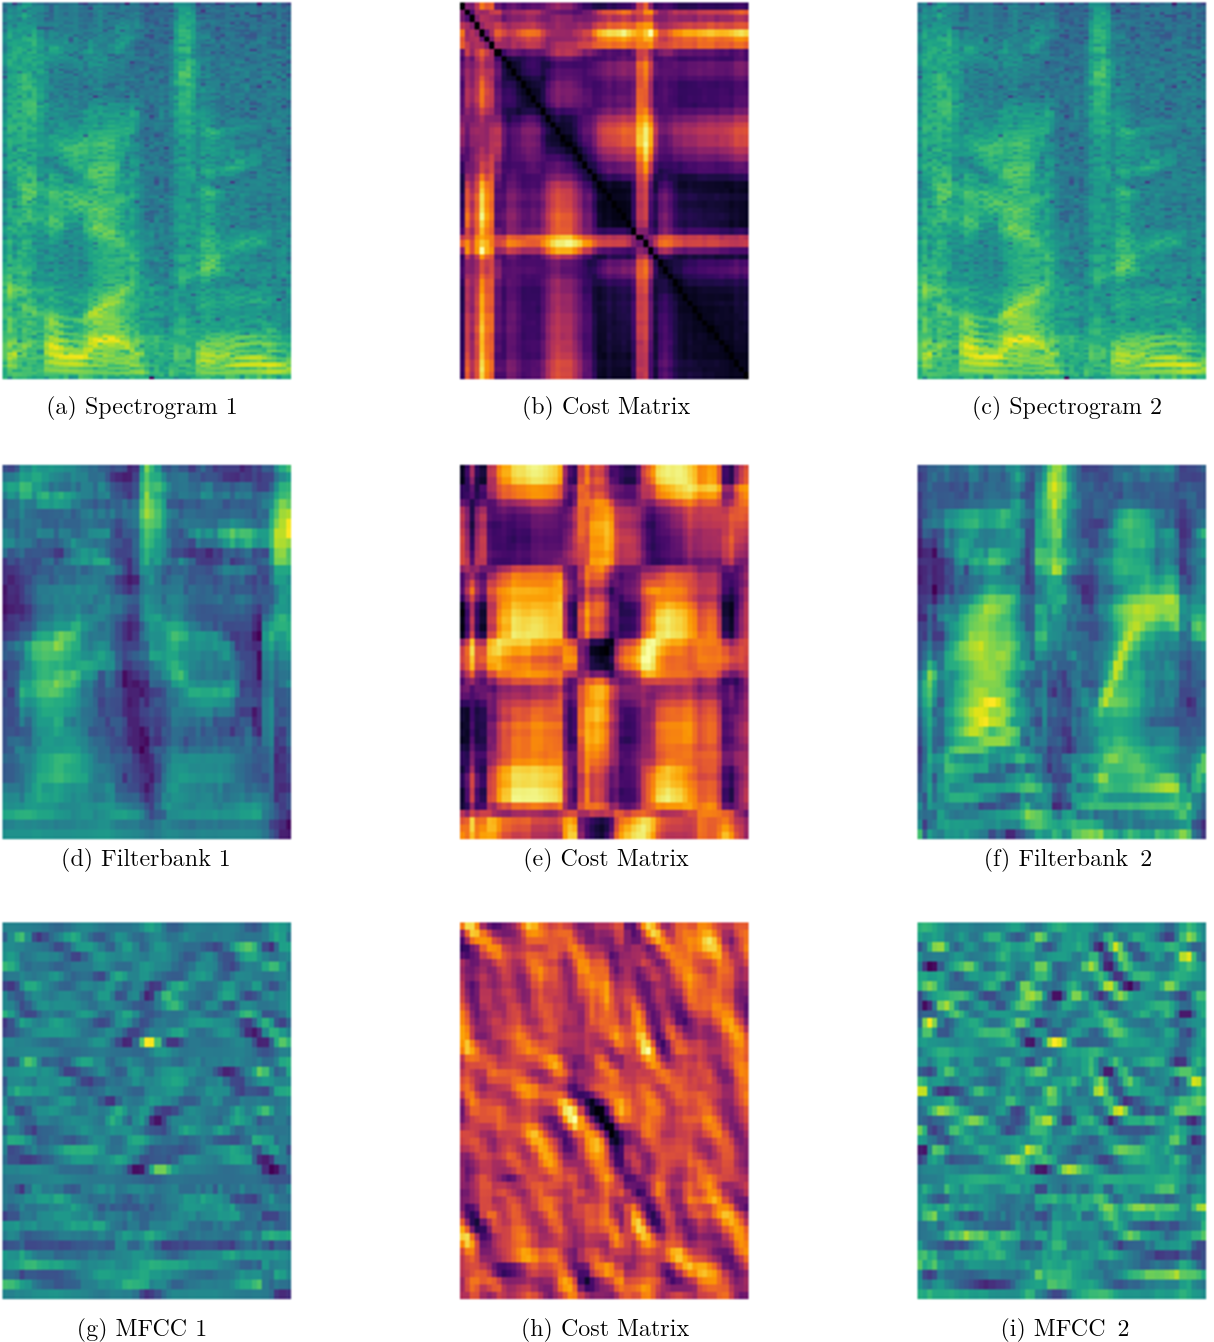
\includegraphics[width=0.9\linewidth]{content/fig/cost_matrices.png}
    \caption{Spectrogram, filterbank and MFCC for two spoken phrases of the word ``graduate" and the distance and cost matrix between each, with lighter colour representing a higher cost.}
    \label{fig:cost_matrix}
\end{figure}

\section{Single Filter Analysis}

Now that our benchmarks have been set, we move on to our first experiment to evaluate the features per individual feature map obtained from the VGG16 network. 
We obtain these features from three input features, namely the spectrograms, filterbanks and MFCCs.
With the features obtained from the spectrogram we at the very least hope to improve our AP score relative to that of the spectrogram benchmark score.
With the features derived from the filterbanks and MFCC we hope to not only improve on the benchmark respective benchmark scores, but also specifically on the MFCC score, thereby improving on existing feature extraction techniques as well as possibly reducing the input vector size.

\subsection{Spectrogram Filters}

When evaluating the feature maps obtained from the spectrograms of the spoken words, we hope to find a feature map that has a more natural distance matrix flow than that of the normal spectrogram, which would ultimately result in a better AP score.
If possible, we hope to find a feature map that outperforms both filterbanks and MFCCs.

The evaluation results, with the top 3 features of each layer shown in Table~\ref{tbl:spectrograms} and all features having an AP score above the spectrogram benchmark shown in Appendix~\ref{appen:ap_scores}, show that there are 167 features that beat the spectrogram benchmark score, with multiple features from every layer in the VGG16 network.
None of the features were able to beat the filterbank or MFCC benchmark, though the top feature, namely \texttt{conv\_2:27}, came within 2\% of the filterbank score, improving upon spectrograms by 691\%.

\begin{table}[!ht]
    \mytable
    \caption{AP scores for the top performing features obtained from spectrograms.}
    \begin{tabularx}{0.85\linewidth}{@{}cLl@{}}
        \toprule
        Rank & Feature        & AP       \\
        \midrule
        11 & 	\texttt{conv1\_1:5} & $0.1106$ \\
        22 & 	\texttt{conv1\_1:16} & $0.0887$ \\
        33 & 	\texttt{conv1\_1:31} & $0.0773$ \\ \hline
        1 & 	\texttt{conv1\_2:27} & $0.1857$ \\
        9 & 	\texttt{conv1\_2:4} & $0.1128$ \\
        15 & 	\texttt{conv1\_2:52} & $0.0955$ \\ \hline
        2 & 	\texttt{conv2\_1:74} & $0.1639$ \\
        6 & 	\texttt{conv2\_1:119} & $0.1196$ \\
        7 & 	\texttt{conv2\_1:90} & $0.1180$ \\ \hline
        3 & 	\texttt{conv2\_2:106} & $0.1613$ \\
        4 & 	\texttt{conv2\_2:6} & $0.1509$ \\
        19 & 	\texttt{conv2\_2:64} & $0.0914$ \\ \hline
        8 & 	\texttt{conv3\_1:119} & $0.1153$ \\
        10 & 	\texttt{conv3\_1:251} & $0.1109$ \\
        12 & 	\texttt{conv3\_1:175} & $0.1066$ \\ \hline
        5 & 	\texttt{conv3\_2:89} & $0.1292$ \\
        16 & 	\texttt{conv3\_2:161} & $0.0950$ \\
        18 & 	\texttt{conv3\_2:143} & $0.0918$ \\ \hline
        20 & 	\texttt{conv3\_3:114} & $0.0910$ \\
        42 & 	\texttt{conv3\_3:88} & $0.0649$ \\
        48 & 	\texttt{conv3\_3:62} & $0.0582$ \\ \hline
        & Benchmark & $0.02347$ \\
        \bottomrule
    \end{tabularx}
    \label{tbl:spectrograms}
\end{table}

Due to these features still being larger vectors than that of filterbanks and MFCCs, it was determined to be an impractical approach to measure combined feature AP scores and thus further increasing the size.
Performing feature extraction on generic spectrograms, though feature quality is improved, can not be a sufficient feature extraction technique when used alone, as it does not reduce feature size enough nor results in a high enough AP score.
Instead, feature extraction was performed on filterbanks and MFCCs in order to obtain at least an equivalent vector size.

\subsection{Filterbank Filters}

For the feature maps obtained from the filterbanks, we hope to find one or more feature maps that beat the AP score of not only the generic filterbank, but also that of the MFCC.
If this feature map could be one obtained from $\mathtt{conv2\_1}$ onward, this would also result in a reduced feature map size whilst improving the feature quality.

When these features were evaluated, the results of which can be seen in Table~\ref{tbl:filterbanks}, it was found that four features outperformed the generic filterbank AP score, with one being from layer $\mathtt{conv2\_1}$, thus halving the input feature and still improving the quality.

It is also interesting to note that none of the features obtained from $\mathtt{conv3\_1}$ were able to beat the benchmark score, suggesting that too small a feature vector may not carry enough information to distinguish words as effectively.

\begin{table}[!ht]
    \mytable
    \caption{AP scores for the top performing features obtained from filterbanks.}
    \begin{tabularx}{0.85\linewidth}{@{}cLl@{}}
        \toprule
        Rank & Feature layer          & AP       \\
        \midrule
        1 & $\mathtt{conv1\_2:9}$     & $0.2363$ \\
        2 & $\mathtt{conv1\_2:26}$    & $0.2287$ \\
        3 & $\mathtt{conv2\_2:27}$    & $0.2148$ \\
        4 & $\mathtt{conv1\_2:53}$    & $0.2124$ \\ \hline
        & Benchmark & $0.1890$ \\
        \bottomrule
    \end{tabularx}
    \label{tbl:filterbanks}
\end{table}
Unfortunately, none of the features obtained were able to beat the MFCC score, but improving upon the generic filterbank score is still a noteworthy achievement, with the top feature improving the AP score by 25\%.
It may also be suggested that the features obtained from layer $\mathtt{conv2\_2:27}$, though not as accurate as MFCCs, could be used for speech recognition where smaller model sizes are required, due to the feature sized being effectively quartered.
We go on to qualitatively examine how these features were able to achieve improved AP scores.

\subsubsection{Qualitative Analysis}

When examining the qualitative properties of the extracted feature maps, shown for the word ``collecting" in Figure~\ref{fig:fbank_features}, there seemed to be a strong tendency within the first, second and fourth feature maps to emphasise frequencies that were gradually rising in time.
This was found to, in most cases, be linked to occurrences where the speaker is switching from a nasal or lateral consonant to a vowel.
This could greatly improve the ability to recognise similar words by more easily recognising similar consonant-to-vowel transitions.

\begin{figure}[ht]
    \centering
    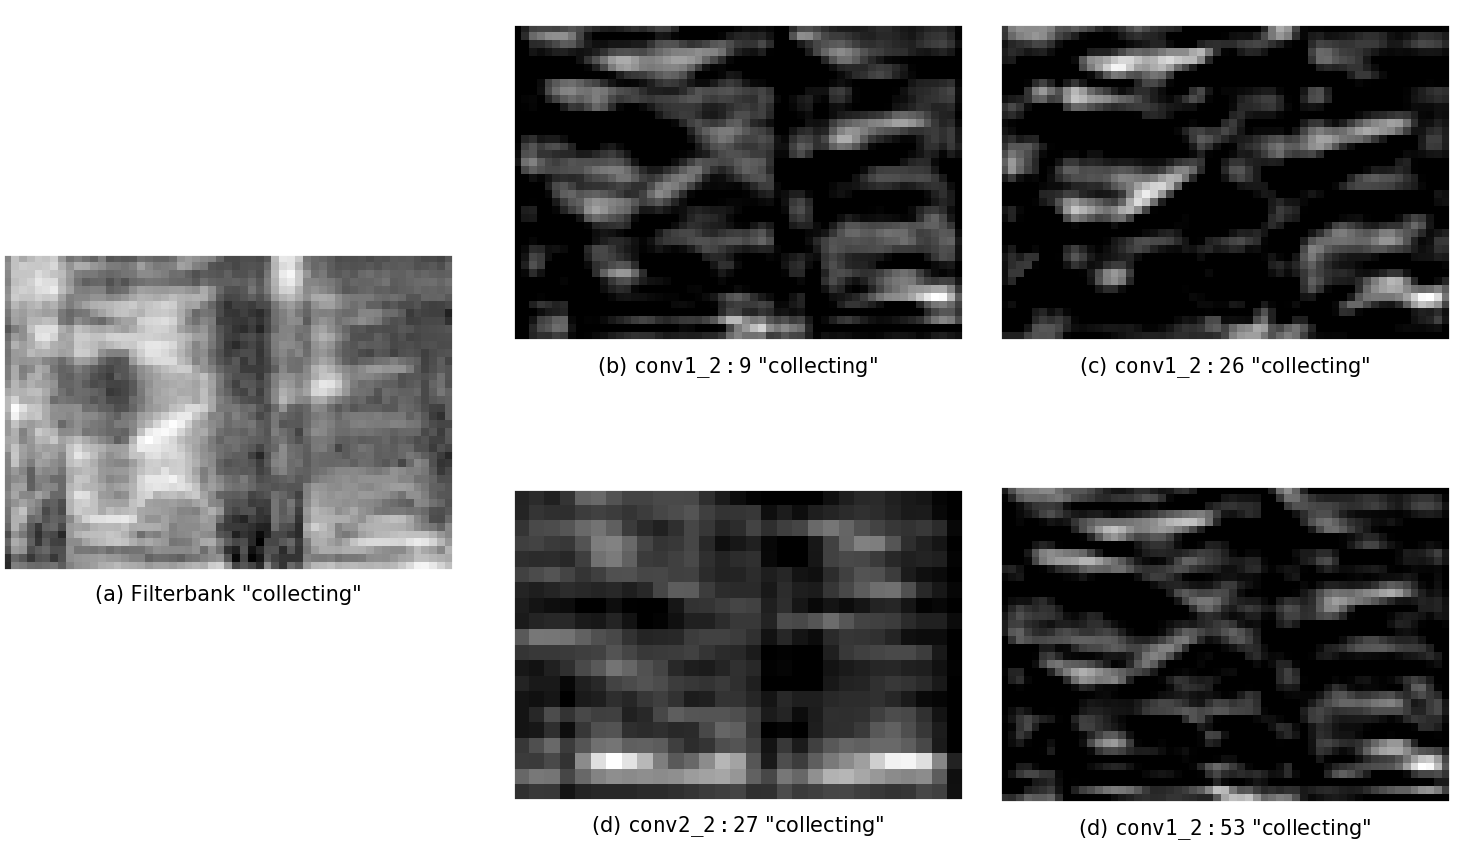
\includegraphics[width=0.5\linewidth]{content/fig/fbank_features.png}
    \caption{The filterbank and corresponding feature maps for the word ``collecting".}
    \label{fig:fbank_features}
\end{figure}

\subsection{MFCC Filters}
\label{chap:mfcc_filters}

For features obtained from the MFCCs, we require that they beat the benchmark score of the MFCC to show any improvement.
If these features could also be obtained from layer $\mathtt{conv2\_1}$ onward, it would also mean that we are able to better represent speech data within a smaller feature vector, greatly improving our feature analysis.

After evaluation, three features were found to beat the MFCC benchmark score, as shown in Table~\ref{tbl:mfccs}. 
Though this does prove our task a success, none of the features were obtained from layer $\mathtt{conv2\_1}$ onward, thus not reducing feature size whilst improving upon quality.

\begin{table}[!ht]
    \mytable
    \caption{AP scores for the top performing features obtained from MFCCs.}
    \begin{tabularx}{0.85\linewidth}{@{}cLl@{}}
        \toprule
        Rank & Feature layer          & AP       \\
        \midrule
        1 & $\mathtt{conv1\_2:17}$    & $0.3064$ \\
        2 & $\mathtt{conv1\_2:37}$    & $0.3007$ \\
        3 & $\mathtt{conv1\_1:9}$     & $0.2960$ \\ \hline
        & Benchmark & $0.2843$ \\
        \bottomrule
    \end{tabularx}
    \label{tbl:mfccs}
\end{table}

In order to try and find a reduced feature input size, we expanded our results to find the top four features obtained from MFCCs from layer $\mathtt{conv2\_1}$ onward that still beat the filterbank benchmark score. These results are shown in Table~\ref{tbl:mfccs2}.
Though these features are of lesser quality than MFCCs, their reduced size may be useful for smaller speech recognition systems that cannot afford such large input vectors.
These features are a quarter the size of the original MFCC input feature, and only reduce the AP score by 16 to 19\%, thus still retaining a fairly high quality.

\begin{table}[!ht]
    \mytable
    \caption{AP scores for the top four performing features obtained from MFCCs from layer $\mathtt{conv2\_1}$ onward.}
    \begin{tabularx}{0.91\linewidth}{@{}cLl@{}}
        \toprule
        Rank & Feature layer          & AP       \\
        \midrule
        1 & $\mathtt{conv2\_1:84}$    & $0.2360$ \\
        2 & $\mathtt{conv2\_1:121}$   & $0.2333$ \\
        3 & $\mathtt{conv2\_1:75}$    & $0.2314$ \\
        4 & $\mathtt{conv2\_1:111}$   & $0.2304$ \\
        \bottomrule
    \end{tabularx}
    \label{tbl:mfccs2}
\end{table}

\subsubsection{Qualitative Analysis}

In order to understand how the top features obtained from the MFCCs improve on its AP score, we look into the qualitative properties of the filters used to obtain these features.

\begin{figure}[h]
    \centering
    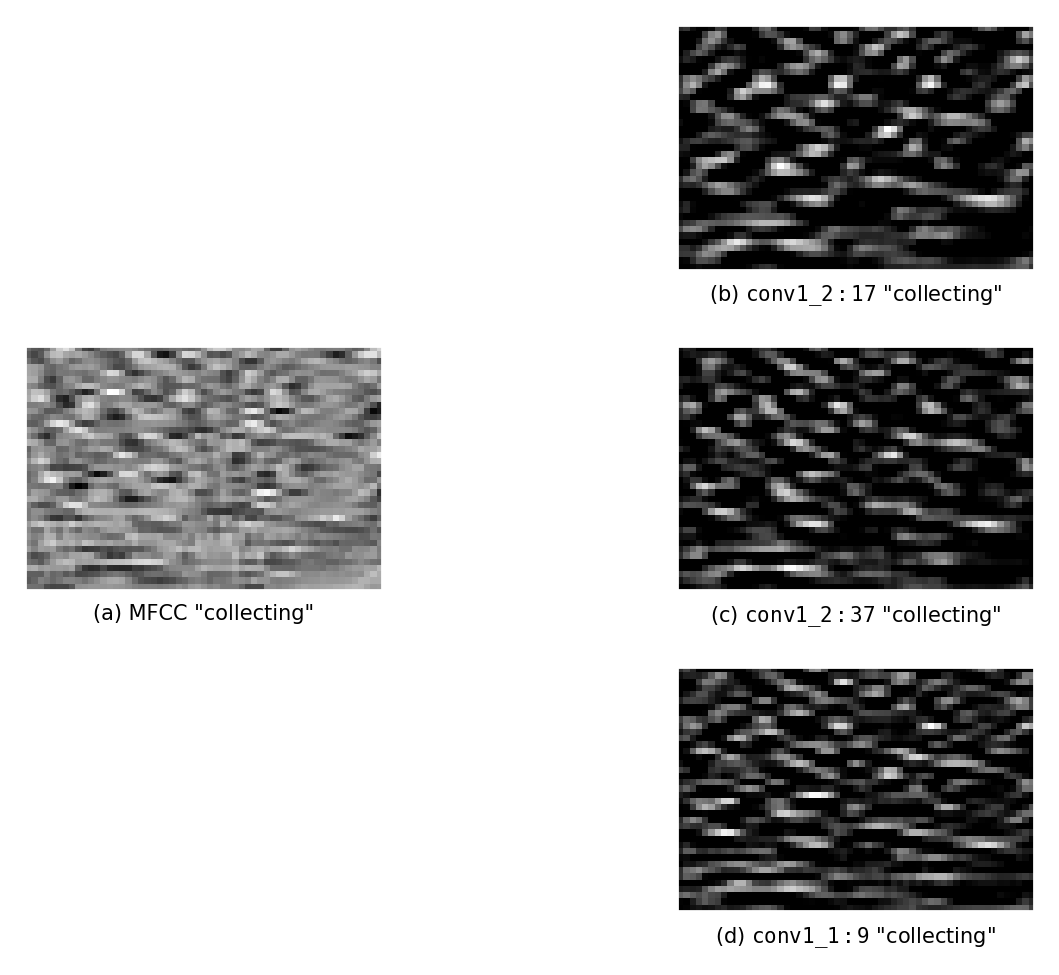
\includegraphics[width=0.5\linewidth]{content/fig/mfcc_features.png}
    \caption{The MFCC and corresponding feature maps for the word ``collecting".}
    \label{fig:mfcc_features}
\end{figure}

Looking at the feature maps extracted for each of these layers for the word ``collecting", shown in Figure~\ref{fig:mfcc_features}, we can see that the top two feature maps are fairly similar.
Upon deeper inspection it was found that these filters act as deeper forms of edge detection, activating over any high spots that are immediately surrounded by fairly low spots.
This has the result of isolating higher volume spots in such a way that it could capture more coherently the parts of speech focused on by humans.
Looking at the third feature map, we can see the filter effect by looking at the filter kernel, shown in Appendix~\ref{appen:conv1_1} ($\mathtt{conv1\_1:9}$).
Keeping in mind that colours are flattened for the speech features, it is clear that the filter kernel also acts as a sort of edge detector, and thus the slight resemblance to the first two feature maps.

\section{Combined Filter Analysis}

In order to try and obtain an even higher AP score whilst retaining feature size, the top four feature maps obtained from the second layer in the VGG16 network ($\mathtt{conv2\_1}$ and $\mathtt{conv2\_2}$) were concatenated to each other to form a single feature map for each of the filterbanks and the MFCCs.
Since the second convolutional layer produces a feature map of size $\frac{N}{2} \times \frac{M}{2}$, with an input feature of size $N \times M$, it in effect quarters the size of the feature.
Thus, concatenating four feature maps from this layer would result in a feature map of size $\frac{N}{2} \times 2M$, which is still the same total size as the original feature vector.
It is the hope that these combined feature maps will each carry different types of information of the spoken word they are derived from, thus acting as a hybrid feature map that performs better than the individual features.

\subsection{Top Filterbank Filters}

For the filterbanks, the top four second layer feature maps are shown in Table~\ref{tbl:fbanks2}.
Though only the top feature actually outperforms filterbanks, it is hoped that each of these features capture a different piece of information of the spoken word and that, if combined, these features will outperform other features.

\begin{table}[!ht]
    \mytable
    \caption{AP scores for the top four features obtained from filterbanks from layer $\mathtt{conv2\_1}$ onward.}
    \begin{tabularx}{0.91\linewidth}{@{}cLl@{}}
        \toprule
        Rank & Feature layer          & AP       \\
        \midrule
        1 & $\mathtt{conv2\_1:27}$    & $0.2148$ \\
        2 & $\mathtt{conv2\_1:15}$   & $0.1754$ \\
        3 & $\mathtt{conv2\_1:62}$    & $0.1479$ \\
        4 & $\mathtt{conv2\_1:1}$   & $0.1479$ \\
        \midrule
        & Combined Features & $0.2622$ \\
        \bottomrule
    \end{tabularx}
    \label{tbl:fbanks2}
\end{table}

An example of this combined filter is shown for the word "collecting" in Figure~\ref{fig:fbank_combined}, which makes it clear how the features are concatenated.

After concatenating all the features, the same AP score algorithm described in Chapter~\ref{chap:evaluation} was run on these features to obtain the AP score shown at the bottom of Table~\ref{tbl:fbanks2}.
Clearly, combining these filters results in a higher AP score than that of the individual filters as well as the benchmark filterbank score.
The combined filters also perform better than any other individual filter obtained from filterbanks, giving merit to the technique of combining top filters.

Unfortunately, the AP score is still 7.8\% lower than that of the MFCC benchmark, but coming this close to the MFCC score certainly provides some evidence that visual feature extraction techniques can be applied to speech data.

\begin{figure}[ht]
    \centering
    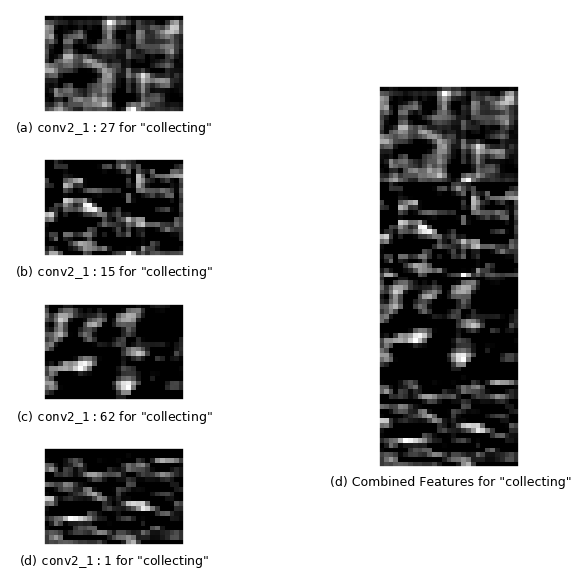
\includegraphics[width=0.5\linewidth]{content/fig/fbankCombined.png}
    \caption{The top four feature maps for the word "collecting" obtained from filterbanks through the second convolutional layer and the combined feature.}
    \label{fig:fbank_combined}
\end{figure}

\subsection{Top MFCC Filters}

Going one step further, we try the same feature combination technique as with filterbanks, combining the top four MFCC feature maps from the second convolutional layer to form a single combined feature.
The AP score of this feature is shown in Table~\ref{tbl:mfcc_combined}.

\begin{table}[!ht]
    \mytable
    \caption{AP score for for the combined feature from the top four features obtained by passing the MFCC through layer $\mathtt{conv2}$.}
    \begin{tabularx}{0.91\linewidth}{@{}Ll@{}}
        \toprule
        Feature layer          & AP       \\
        \midrule
        Combined Feature    & $0.2906$ \\
        \bottomrule
    \end{tabularx}
    \label{tbl:mfcc_combined}
\end{table}

Comparing the AP score to that of the individual features in Table~\ref{tbl:mfccs2} shows that the combined feature yet again outperforms the individual filters as well as the MFCC benchmark.
Unfortunately, it is not able to outperform the top single filter features, falling short by just 5.1\%.

It might be that, as stated in Chapter~\ref{chap:mfcc_filters}, because the properties obtained from the top four features are fairly similar, that combining these specific filters was not as efficient.
There may lie some combination of features that outperform all of the features extracted so far, but due to processing capacity and time limits, this could not be implemented within this study.

\section{Summary of Results}

To summarise the results found in these experiments, Table~\ref{tbl:summarised_results} shows all the top results obtained in a summarised table and the precision-recall curves for all features are shown in Figure~\ref{fig:pr_curves}.
From this Table~\ref{tbl:summarised_results} it is clear that \texttt{conv1\_2:17}, when ran across the MFCC features, is the highest scoring feature, improving the top benchmark score by 7.8\%.

\begin{table}[!ht]
    \mytable
    \caption{Summary of AP Scores for for benchmark features, single filter features per input feature, and combined filter results.}
    \begin{tabularx}{0.91\linewidth}{@{}lcLcl@{}}
        \toprule
        Group       & Rank    & Feature       & Size  & AP Score   \\ \midrule
        Benchmark   & 15 & Spectrograms  & $201 \times N$  & $0.02347$ \\
                    & 11 & Filterbanks   & $40 \times N$  & $0.1890$ \\
                    & 5 & MFCCs         & $39 \times N$  & $0.2843$ \\ \hline
        Spectrogram & 12 & \texttt{conv1\_2:27} & $201 \times N$  & $0.1857$ \\
                    & 13 & \texttt{conv2\_1:74} & $101 \times \frac{N}{2}$  & $0.1639$ \\
                    & 14 & \texttt{conv2\_2:106} & $101 \times \frac{N}{2}$ & $0.1613$ \\ \hline
        Filterbanks & 7 & $\mathtt{conv1\_2:9}$  & $40 \times N$  & $0.2363$ \\
                    & 8 & $\mathtt{conv1\_2:26}$  & $40 \times N$  & $0.2287$ \\
                    & 9 & $\mathtt{conv2\_2:27}$  & $20 \times \frac{N}{2}$  & $0.2148$ \\
                    & 10 & $\mathtt{conv1\_2:53}$  & $40 \times N$  & $0.2124$ \\ \hline
        MFCCs       & \textbf{1} & \texttt{\textbf{conv1\_2:17}}  & $\bm{39 \times N}$  & $\bm{0.3064}$ \\
                    & 2 & $\mathtt{conv1\_2:37}$  & $39 \times N$  & $0.3007$ \\
                    & 3 & $\mathtt{conv1\_1:9}$  & $39 \times N$  & $0.2960$ \\ \hline
        Combined    & 6 & Filterbanks   & $80 \times \frac{N}{2}$  & $0.2622$ \\
                    & 4 & MFCCs         & $78 \times \frac{N}{2}$  & $0.2906$ \\
        \bottomrule
    \end{tabularx}
    \label{tbl:summarised_results}
\end{table}

Some other noteworthy results are the \texttt{conv2\_2:27} feature obtained from the filterbanks, a feature that improves in quality from filterbanks, whilst quartering the feature size.
Another is the combined filterbank feature, providing even better AP scores than any other individual filter obtained from filterbanks.

\begin{figure}[!h]
    \centering
    
\includegraphics[width=0.95\linewidth]{content/fig/pr_all.png}
    \caption{Combined precision-recall curves for all features obtained from (a) spectrograms, (b) filterbanks and (c) MFCCs.}
    \label{fig:pr_curves}
\end{figure}